\documentclass[../main.tex]{subfiles}
\begin{document}
\subsection*{Appendix}
\subsubsection*{Relativistic kinematics.} For first example, we will discuss relativistic collision. In relativity an isolated system always conserves both momentum and energy. 
\begin{quote}
    Two lumps of clay, each of (rest) mass $m$, collide head-on at $3/5 c$. They stick together. Question: what is the mass (M) of the composite lump?
\end{quote}
In this case conservation of momentum is trivial: zero before, zero after. The energy of each lump prior to the collision is
\begin{equation*}
    \frac{mc^2}{\sqrt{1 - (3/5)2}}=\frac{4}{5}mc^2
\end{equation*}
and the energy of the composite lump after the collision is $M^c2$ (since it's at rest). So conservation of energy says
\begin{equation*}
    \frac{4}{5}mc^2+\frac{4}{5}mc^2=Mc^2
\end{equation*}
and hence
\begin{equation*}
    M=\frac{5}{2}m
\end{equation*}
Thus collision mass is greater than the sum of the initial masses, because mass was not conserved in this collision; kinetic energy was converted into rest energy, so the mass increased.
\begin{figure*}[b]
    \centering
    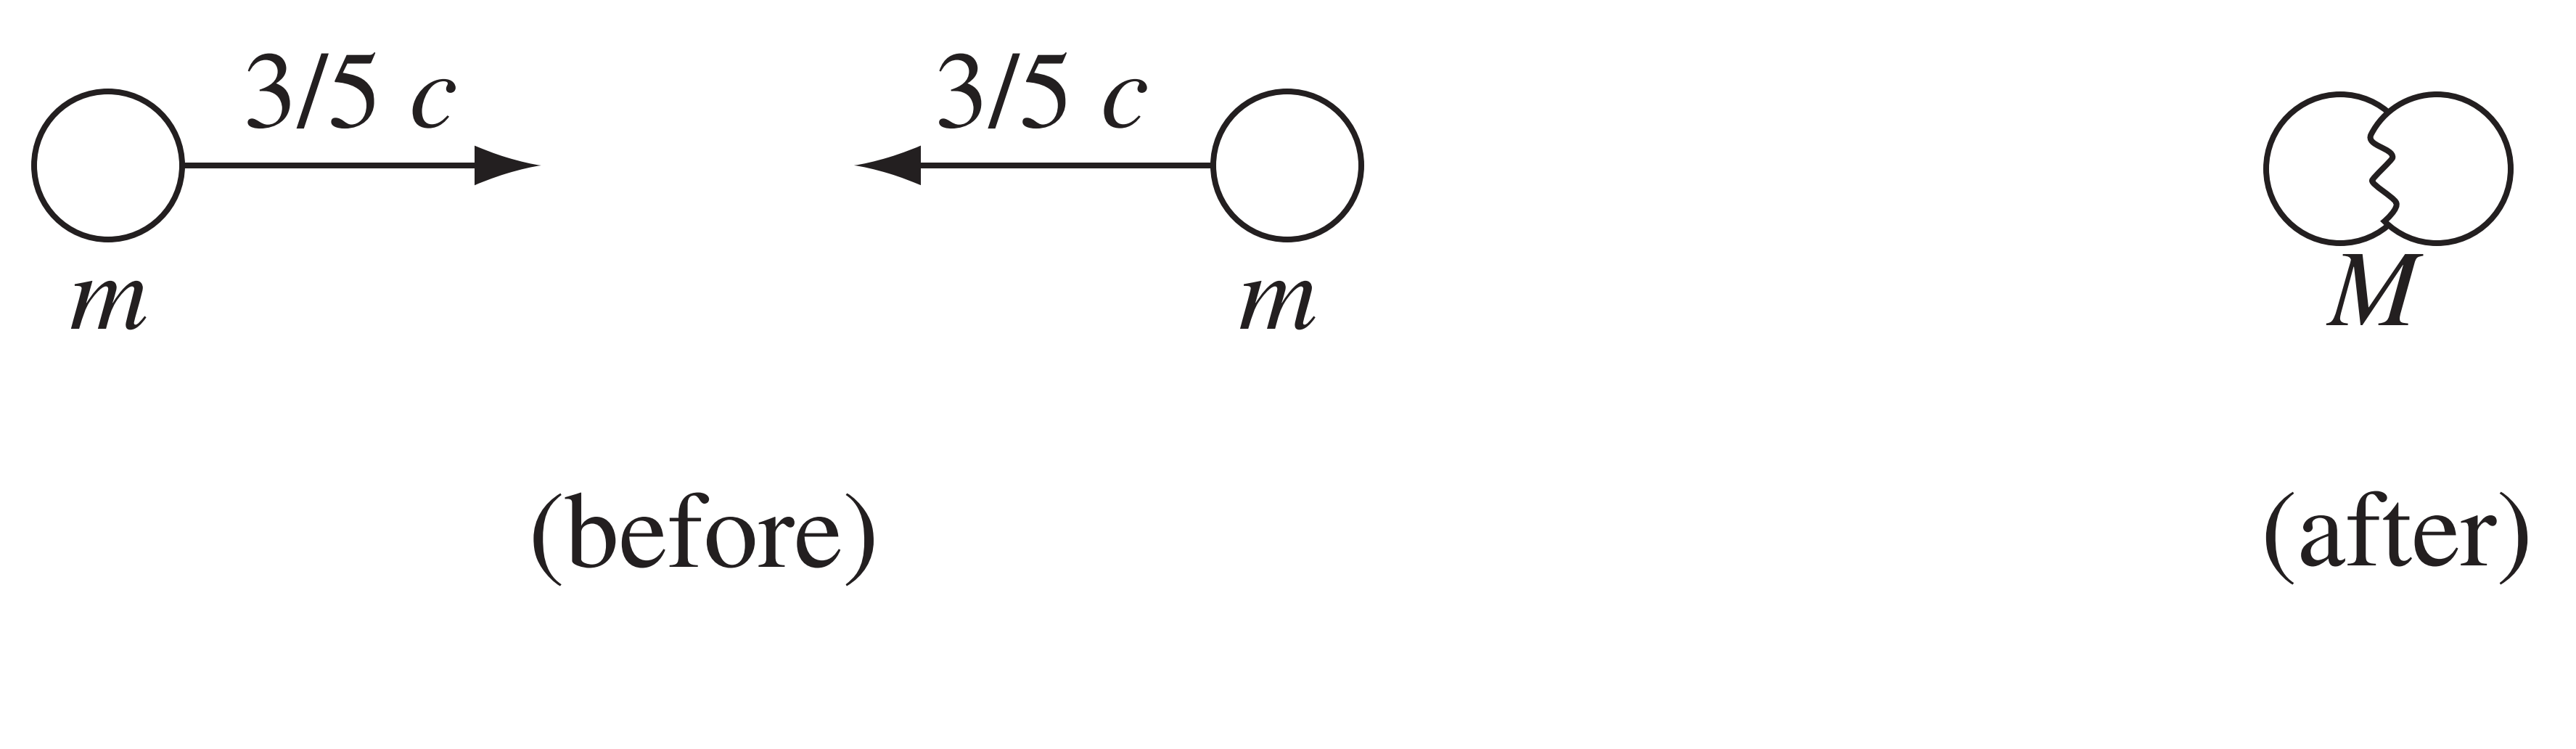
\includegraphics[width=0.75\textwidth]{../Rss/Relativity/Appendix/Collision.png}
    \caption*{Figure: Inelastic collision, which (Classicaly) defined as a collision in which energy is not conserved, but momentum does.}
\end{figure*}

\subsubsection*{Pair creation.} Next example will discuss pair creation. 
\begin{quote}
    A pion at rest decays into a muon and a neutrino. Find the energy of the outgoing muon, in terms of the two masses, $m_\pi$ and $m_\mu$ (assume $m_v = 0$)
\end{quote}
In this case,
\begin{align*}
    E_{\text{before}}&=m_\pi c^2&&\mathbf{p}_{\text{before}}=0\\
    E_{\text{after}}&=E_\mu+E_v&&\mathbf{p}_{\text{after}}=\mathbf{p}_\mu+\mathbf{p}_v
\end{align*}
Conservation of momentum requires that$ \mathbf{p}_v = -\mathbf{p}_\mu$. Conservation of energy says that
\begin{equation*}
   E_\mu+E_v= m_\pi c^2
\end{equation*}
Now, $E_v = |\mathbf{p}_v |c$ and $| \mathbf{p}_\mu |=\sqrt{E_\mu^2-m^2_\mu c^4}/c$. So,
\begin{align*}
    E_\mu+\sqrt{E_\mu^2-m^2_\mu c^4}&=m_\pi c^2\\
    \sqrt{E_\mu^2-m^2_\mu c^4}&=m_\pi c^2-E_\mu\\
    E_\mu^2-m^2_\mu c^4&=E_\mu^2+m_\pi^2 c^4-2E_\mu m_\pi c^2\\
    2E_\mu m_\pi c^2&=(m_\pi^2+m^2_\mu)c^4\\
    E_\mu&=\frac{(m^2_\pi+m^2_\mu)c^2}{2m_\pi}
\end{align*}
We call the collision elastic if kinetic energy is conserved. In such a case the rest energy (being the total minus the kinetic) is also conserved, and therefore so too is the mass. In practice, this means that the same particles come out as went in. 
\begin{figure*}[t]
    \centering
    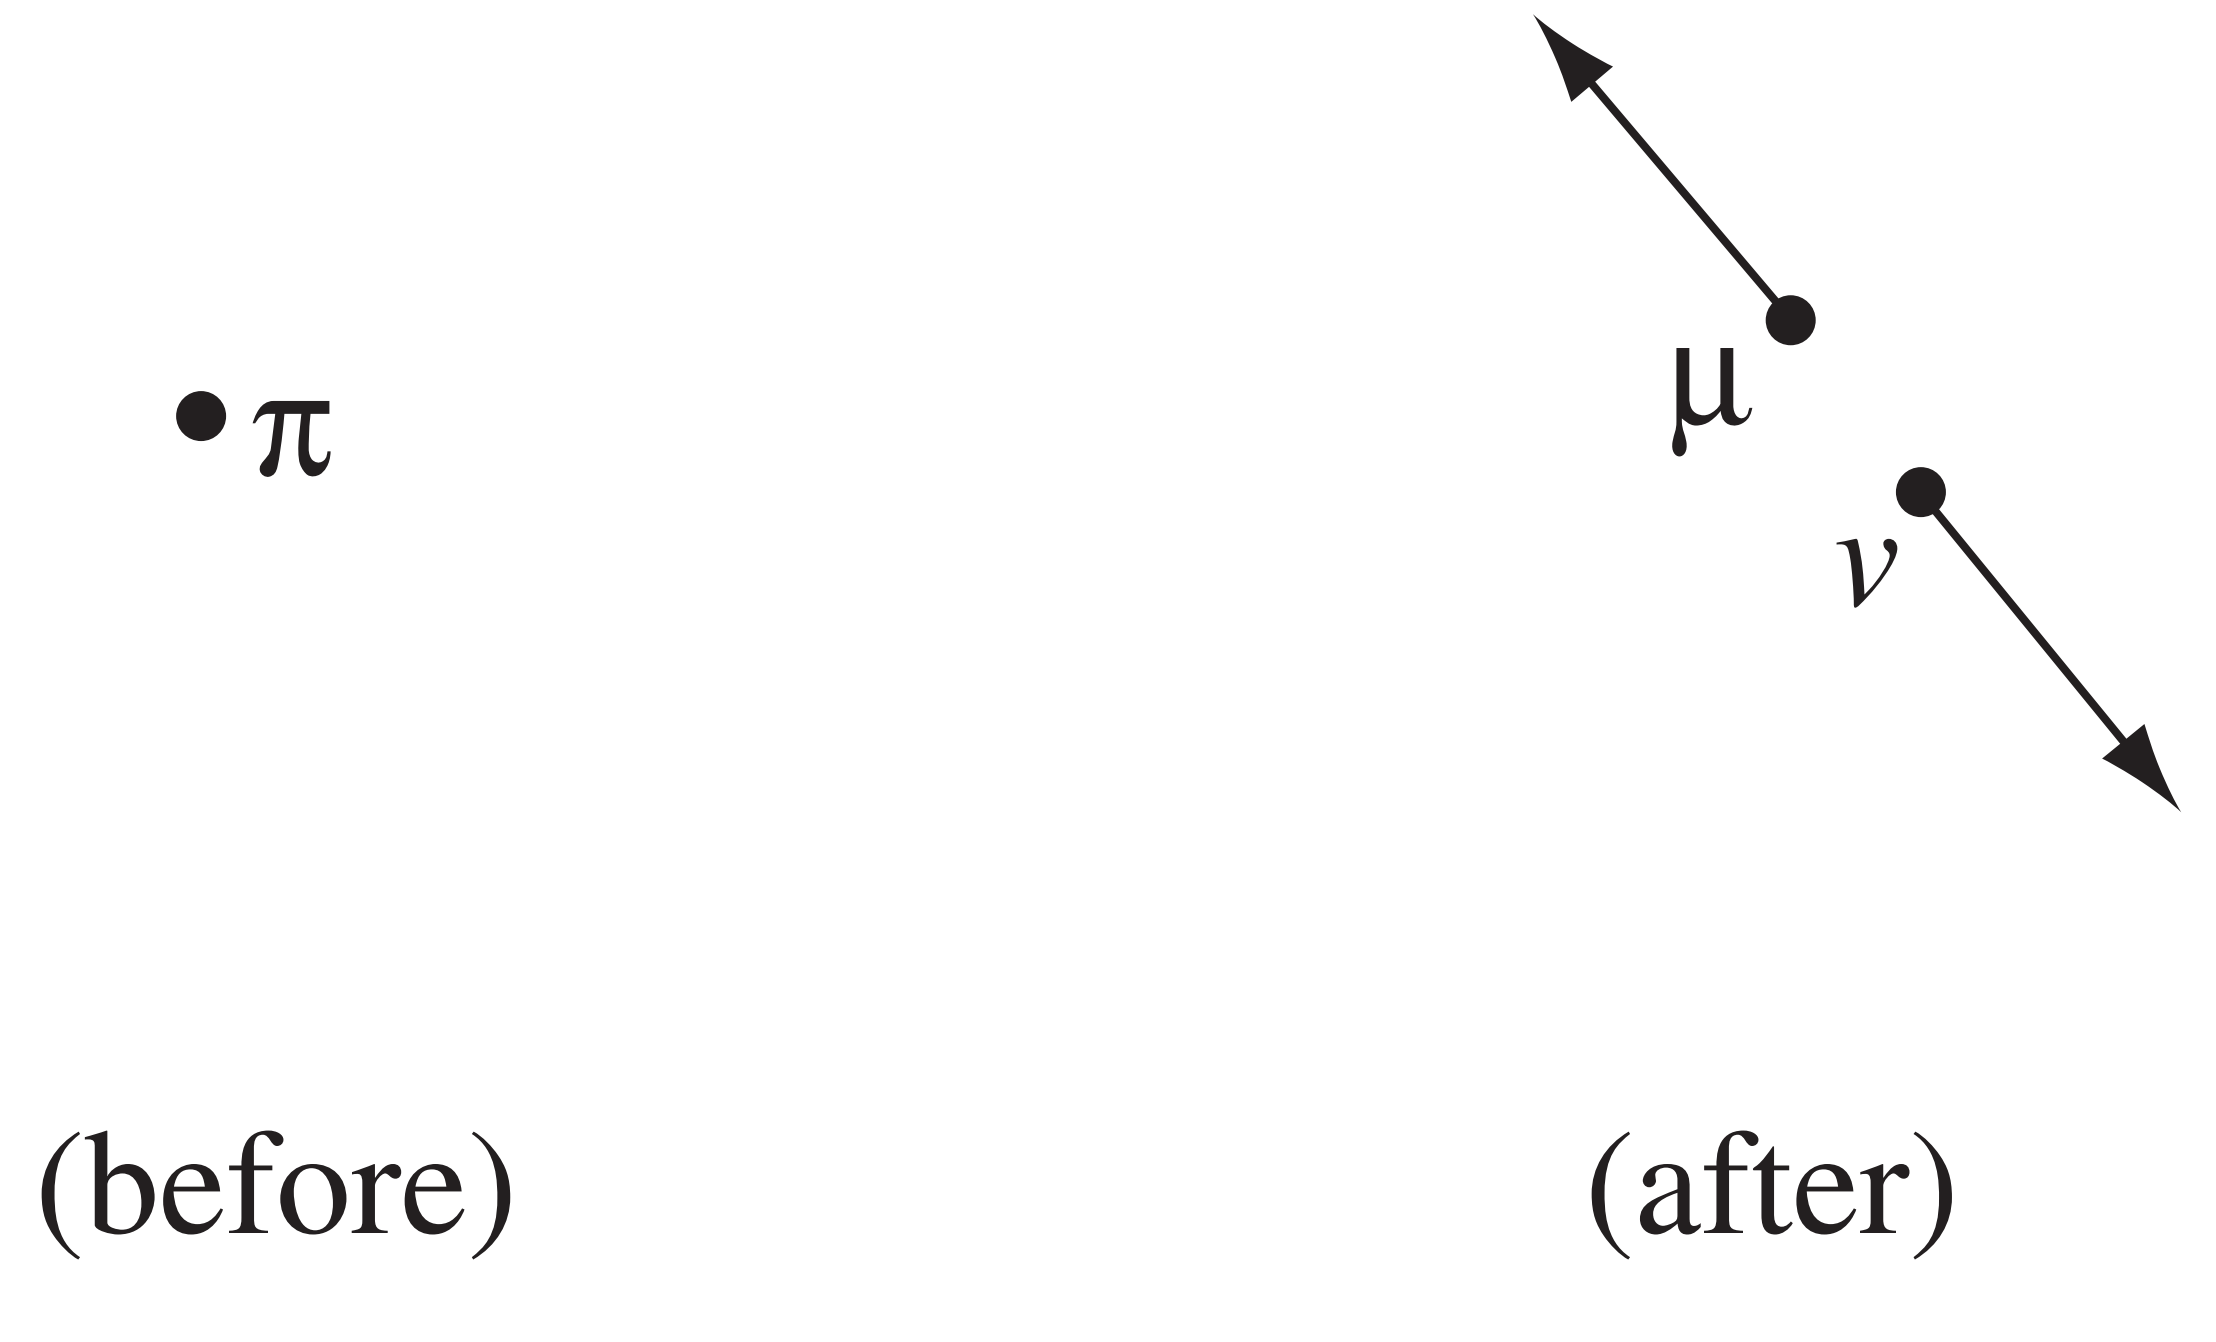
\includegraphics[height=3cm]{../Rss/Relativity/Appendix/PairCreation.png}
    \caption*{Figure: Pair Creation}
\end{figure*}

\subsubsection*{Compton scattering.} Those two examples were inelastic processes; the next one is elastic.
\begin{figure*}[b]
    \centering
    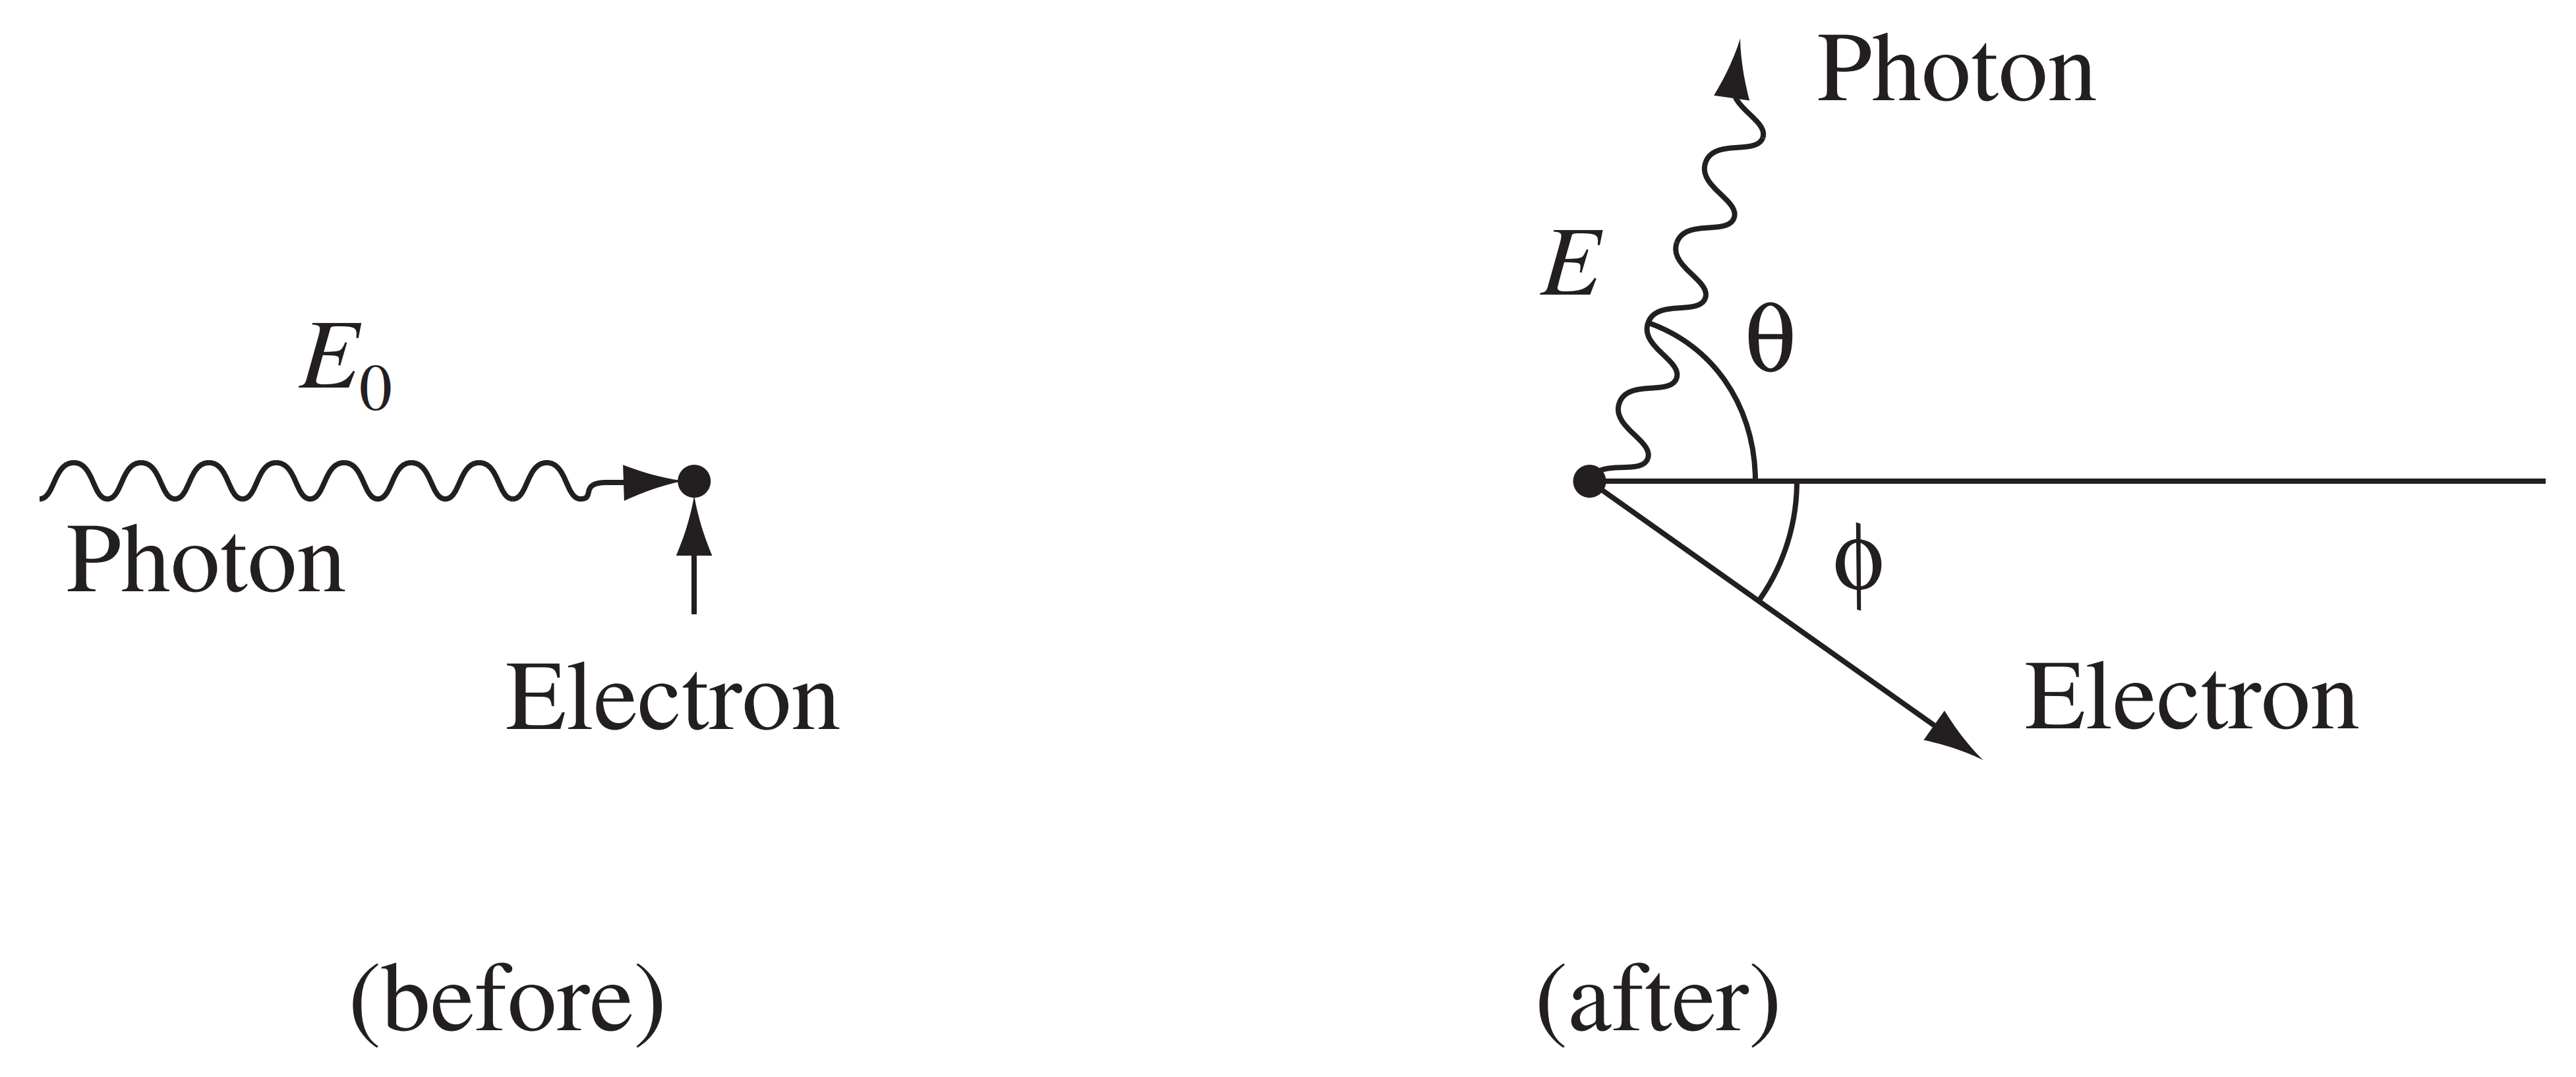
\includegraphics[width=0.75\textwidth]{../Rss/Relativity/Appendix/Compton.png}
    \caption*{Figure: Pair Creation}
\end{figure*}

\begin{quote}
    A photon of energy $E_0$ “bounces” off an electron, initially at rest. Find the energy $E$ of the outgoing photon, as a function of the scattering angle $\theta$ 
\end{quote}
Conservation of momentum in the “vertical” direction gives $p_e \sin \phi = p_p \sin \theta$. Since $p_p = E/c$
\begin{equation*}
    \sin \phi=\frac{E}{c p_e}\sin \theta
\end{equation*}
Conservation of momentum in the “horizontal” direction gives
\begin{align*}
    \frac{E_0}{c}&=p_p \cos \theta + p_e \cos \phi\\
    &=\frac{E}{c}\cos \theta+ p_e \sqrt{1-(\frac{E}{c p_e}\sin \theta)^2}\\
    (E_0-E\cos\theta)^2&=p_e^2c^2-E^2\sin\theta\\
    p_e^2c^2&=E_0^2+E_0^2\cos^2\theta-2EE_0\cos\theta+E_0^2\sin^2\theta\\
    &=E^2+E_0^2-2EE_0\cos\theta
\end{align*}
where $ \cos \phi$ obtained from Phytagorean identity. Finally, conservation of energy says that
\begin{align*}
    E_0 + mc^2& = E + E_e \\
    &=E+ \sqrt{m^2c^4 + p^2_e c^2}\\
    &=E+ \sqrt{m^2c^4 + E^2+E_0^2-2EE_0\cos\theta}
\end{align*}
Next, we solve for $E$
\begin{equation*}
    (E_0-E)^2=E^2 + E_0^2 + m^2c^4 +E_0^2-2EE_0\cos\theta
\end{equation*}
expanding the term in parenthesis
\begin{multline*}
    E^2 + E_0^2 + m^2c^4 - 2EE_0-2Emc^2 + 2E_0mc^2\\=E^2 + E_0^2 + m^2c^4 +E_0^2-2EE_0\cos\theta
\end{multline*}
The first three terms cancel, thus
\begin{equation*}
    - 2EE_0-2Emc^2 + 2E_0mc^2=-2EE_0\cos\theta
\end{equation*}
Finally,
\begin{align*}
    \frac{mc^2}{E}-\frac{mc^2}{E_0}-1=-\cos\theta\\
    \frac{E}{mc^2}=\frac{1}{1-\cos\theta+mc^2/E_0}\\
    E=\frac{1}{(1-\cos\theta)/mc^2+1/E_0}
\end{align*}
The answer looks nicer when expressed in terms of photon wavelength
\begin{equation*}
    E=hv=\frac{h\lambda}{c}
\end{equation*}
Then,
\begin{align*}
    \frac{hc}{\lambda}&=\frac{1}{(1-\cos\theta)/mc^2+\lambda_0/hc}\\
    \frac{\lambda}{hc}&=\frac{1}{mc^2}(1-\cos\theta)+\frac{\lambda_0}{hc}\\
\end{align*}
So
\begin{equation*}
    \lambda=\lambda_0+\frac{h}{mc}(1-\cos\theta)
\end{equation*}
The quantity $ (h/mc)$ is called the Compton wavelength of the electron. 
\end{document}